%\vspace{1cm}
\section*{Introducción}
En este documento se muestran problemas en variedad de temas y de dificultad variable. Adicional a estos problemas se recomienda dar un vistazo a diferentes \href{https://drive.google.com/drive/folders/17I-6L5ZBXA8nkakkQ815Gt2cxKC3Ai3m?usp=sharing}{exámenes} de años anteriores en olimpiadas como la \textit{Olimpiada Centroamericana y del Caribe de Física} (OCCAFI), \textit{Olimpiada Iberoamericana de Física} (OIbF), \textit{International Physics Olimpiad} (IPhO), \textit{Olimpiada Interuniversitaria de Guatemala}, etc.

\section*{Vectores}
\begin{ejercicio}
	Resuelva los siguientes incisos.
	\begin{itemize}
		\item Encuentre el ángulo entre las diagonales de las caras contigüas de un cubo.
		\begin{center}
			


\tikzset{every picture/.style={line width=0.75pt}} %set default line width to 0.75pt        

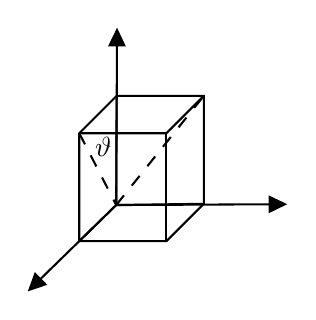
\begin{tikzpicture}[x=0.75pt,y=0.75pt,yscale=-1,xscale=1]
%uncomment if require: \path (0,300); %set diagram left start at 0, and has height of 300

%Shape: Cube [id:dp6038747680393932] 
\draw   (350,136) -- (368,118) -- (410,118) -- (410,170) -- (392,188) -- (350,188) -- cycle ; \draw   (410,118) -- (392,136) -- (350,136) ; \draw   (392,136) -- (392,188) ;
%Straight Lines [id:da6829094301047849] 
\draw    (368,118) -- (367.8,170.6) ;
%Straight Lines [id:da36124944068918086] 
\draw    (367.8,170.6) -- (410,170) ;
%Straight Lines [id:da004458006903363065] 
\draw    (367.8,170.6) -- (350,188) ;
%Straight Lines [id:da21943316361290965] 
\draw  [dash pattern={on 4.5pt off 4.5pt}]  (367.8,170.6) -- (410,118) ;
%Straight Lines [id:da569309436281727] 
\draw  [dash pattern={on 4.5pt off 4.5pt}]  (350,136) -- (367.8,170.6) ;
%Straight Lines [id:da7593701970272995] 
\draw    (367.8,170.6) -- (368.19,88.2) ;
\draw [shift={(368.2,85.2)}, rotate = 90.27] [fill={rgb, 255:red, 0; green, 0; blue, 0 }  ][line width=0.08]  [draw opacity=0] (8.93,-4.29) -- (0,0) -- (8.93,4.29) -- cycle    ;
%Straight Lines [id:da0012548071934168625] 
\draw    (367.8,170.6) -- (447.2,170.21) ;
\draw [shift={(450.2,170.2)}, rotate = 179.72] [fill={rgb, 255:red, 0; green, 0; blue, 0 }  ][line width=0.08]  [draw opacity=0] (8.93,-4.29) -- (0,0) -- (8.93,4.29) -- cycle    ;
%Straight Lines [id:da2187449744897081] 
\draw    (367.8,170.6) -- (327.35,210.1) ;
\draw [shift={(325.2,212.2)}, rotate = 315.68] [fill={rgb, 255:red, 0; green, 0; blue, 0 }  ][line width=0.08]  [draw opacity=0] (8.93,-4.29) -- (0,0) -- (8.93,4.29) -- cycle    ;

% Text Node
\draw (356.2,136.6) node [anchor=north west][inner sep=0.75pt]    {$\vartheta $};


\end{tikzpicture}

		\end{center}
		\item Encuentre el ángulo mostrado en la figura.
		\begin{figure}[H]
			\centering
			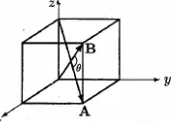
\includegraphics[scale=0.5]{./img/cube.png}
		\end{figure}
	\end{itemize}
\end{ejercicio}



\begin{ejercicio}
	Utilice el producto cruz para encontrar las componentes del vector unitario $\vu{n}$ perpendicular a una de las caras del tetraedro de la siguiente figura:
	\begin{figure}[H]
		\centering
		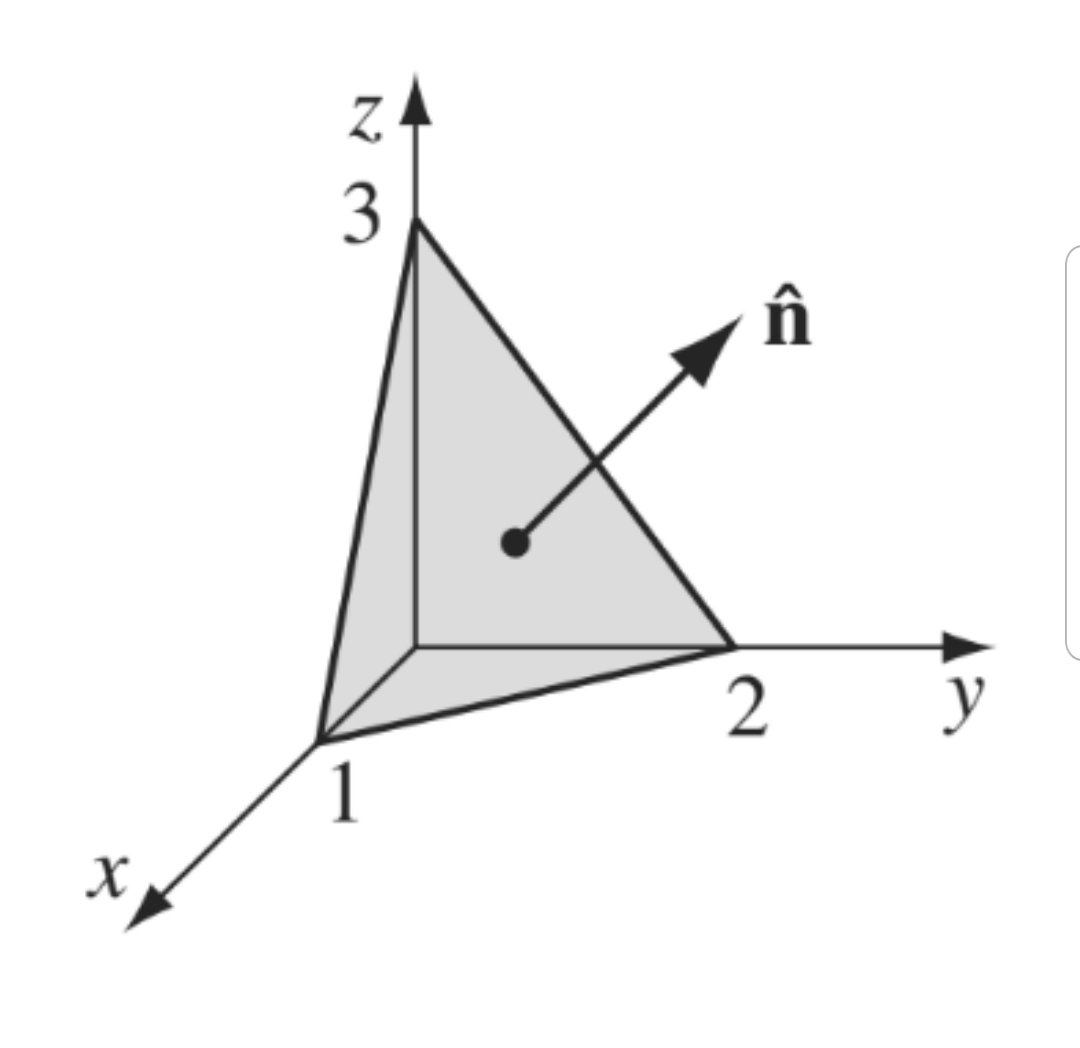
\includegraphics[scale=0.07]{./img/tetraedro.jpeg}
		\caption{Tetraedro.}
		\label{tetraedro}
	\end{figure}
\end{ejercicio}


\section*{Cinemática}


\begin{ejercicio}
	El maquinista de un tren que se mueve a una velocidad $v_1$, advierte la presencia de un tren de carga a una distancia $d$ delante de el que se mueve en la misma vía y en la misma dirección a una velocidad más lenta $v_2$. Acciona los frenos e imprime en su tren una asceleración constante $a$. Demuestre que:
			$$ \text{si} \quad d > \frac{(v_1 - v_2)^2}{2a} \quad \text{no habrá colisión;} $$
			$$ \text{si} \quad d < \frac{(v_1 - v_2)^2}{2a} \quad \text{habrá colisión.} $$
\end{ejercicio}



\begin{ejercicio}
		Spiderman se cae desde la parte más alta de un edificio. Si recorre la segunda mitad del edificio en $1s$, ¿Cuál es la altura del edificio?
\end{ejercicio}



\begin{ejercicio}
	Del orificio de una manguera brotan dos chorros de agua bajo los ángulos $\alpha$ y $\beta$, respecto a la horizontal, con la misma velocidad inicial $v$. ¿A qué distancia horizontal los chorros se intersectan?
	\begin{figure}[H]
		\centering
		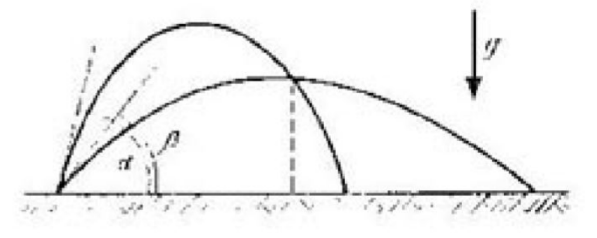
\includegraphics[scale=0.3]{./img/chorros.png}
	\end{figure}
\end{ejercicio}



\begin{ejercicio}
	Una bola es lanzada hacia arriba de un plano con rapidez $v_o$. El plano esta inclinado con respecto a la horizontal un ángulo $\phi$ y la velocidad inicial de la bola forma un ángulo $\theta$ con el plano. Encuentre la distancia, medida a lo largo del plano inclinado, del punto de lanzamiento al punto donde la bola golpea el plano. Y muestre que para un $v_o$ y un $\phi$ dados, la distancia máxima de la bola es
		$$ R_{max} = \frac{v_o ^2}{g(1 + \sin{\phi})}. $$
\end{ejercicio}




\section*{Dinámica}

\begin{ejercicio}
		Si un bloque cuadrado se desliza por una cuña con ángulo recto inclinada un ángulo $\theta$. El coeficiente de fricción cinético entre la cuña y el bloque es $\mu _k$. ¿Cuál es la aceleración del bloque en términos de las variables conocidas?
		\begin{figure}[H]
			\centering
			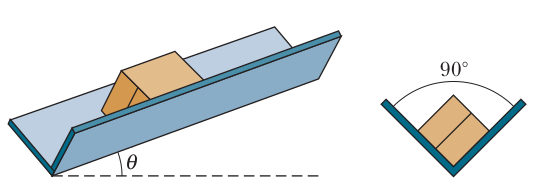
\includegraphics[scale=0.3]{./img/cuna.png}
		\end{figure}
	\end{ejercicio}



\begin{ejercicio}
		En la figura se muestra un sistema mecánico que consiste en tres carritos, $A$, $B$ y $C$ de masas $m_1$, $m_2$ y $m_3$ respectivamente. Los carros $A$ y $B$ estan conectados por una cuerda ligera e inelástica que pasa por una polea ideal fijada en $C$. Para este problema se ignora la fuerza de fricción.
	\begin{enumerate}
		\item Una fuerza horizontal $\vec{F}$ es aplicada al carro $C$. El tamaño de $\vec{F}$ es tal qeu los carritos $A$ y $B$ se mantienen en reposo respecto al carro $C$.
		\begin{enumerate}[a)]
			\item Encuentre la tensión de la cuerda que conecta los carritos $A$ y $B$.
			\item Determine la magnitud de $\vec{F}$.
		\end{enumerate}
		\item Luego, el carro $C$ se detiene. Mientras que los carritos $A$ y $B$ se sueltan desde el reposo.
		\begin{enumerate}[a)]
			\item Determine las aceleraciones de los carritos $A$ y $B$.
			\item Calcule la tensión de la cuerda.
		\end{enumerate}
	\end{enumerate}
		\begin{figure}[H]
			\centering
			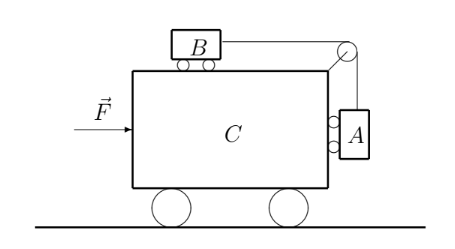
\includegraphics[scale=0.4]{./img/carrito.png}
		\end{figure}
	\end{ejercicio}






\section*{Energía}



\begin{ejercicio}
		Un bloque de masa $m$ se desliza sin roce por una rampa cuya forma está definida por la ecuación:
			$$ \qty[\frac{x - a}{a}]^2 + \qty[\frac{y - b}{b}]^2 = 1. $$
		La partícula parte desde el reposo en el punto $A$ y al alcanzar el punto $B$ sigue deslizando sobre una superficie horizontal rugosa de largo $d$ para finalmente chocar con la plataforma de masa despreciable que está fija a dos resortes, como se indica en la figura. Como resultado del impacto, la partícula se detiene cuando los resortes se comprimen una distancia $\Delta x$. Considerando que la constante elástica de ambos resortes es $k$, calcule el coeficiente de roce cinético $\mu$ que debe existir entre la partícula y la superficie horizontal.
		\begin{figure}[H]
			\centering
			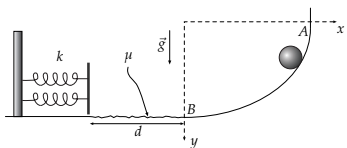
\includegraphics[scale=0.5]{./img/p1.png}
		\end{figure}
	\end{ejercicio}





\begin{ejercicio}
		El clavo $\mathcal{O}'$ está situado a una distancia $d$ por debajo el punto de amarre, $\mathcal{O}$, de la cuerda. Encuentre el valor de $d$ en términos de la longitud de la cuerda, $L$, para que la bola complete una vuelta exacta en un círculo alrededor del clavo.
		\begin{figure}[H]
			\centering
			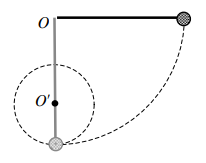
\includegraphics[scale=0.5]{./img/p2.png}
		\end{figure}
	\end{ejercicio}










\section*{Momento Lineal}

\begin{ejercicio}
		Una masa $m_1$ con velocidad $v_o$, golpea un sistema masa resorte $m_2$ inicialmente en reposo. El resorte no tiene masa y tiene una constante $k$. No hay fricción. \\
		\begin{center}
			


\tikzset{every picture/.style={line width=0.75pt}} %set default line width to 0.75pt        

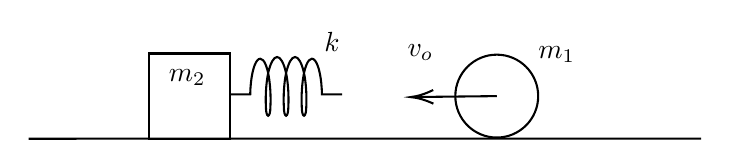
\begin{tikzpicture}[x=0.75pt,y=0.75pt,yscale=-1,xscale=1]
%uncomment if require: \path (0,307); %set diagram left start at 0, and has height of 307

%Straight Lines [id:da2006634064610846] 
\draw    (139,181) -- (463,180.94) ;
%Shape: Rectangle [id:dp9899626707813869] 
\draw   (197,139.94) -- (236,139.94) -- (236,181) -- (197,181) -- cycle ;
%Shape: Circle [id:dp16970128247733873] 
\draw   (344.54,160.47) .. controls (344.54,149.44) and (353.47,140.5) .. (364.5,140.5) .. controls (375.53,140.5) and (384.46,149.44) .. (384.46,160.47) .. controls (384.46,171.5) and (375.53,180.43) .. (364.5,180.43) .. controls (353.47,180.43) and (344.54,171.5) .. (344.54,160.47) -- cycle ;
%Shape: Inductor (Air Core) [id:dp8465340354701729] 
\draw   (236,159.65) -- (245.72,159.65) .. controls (245.86,152.05) and (247.21,145.55) .. (249.12,143.28) .. controls (251.03,141.01) and (253.11,143.43) .. (254.36,149.37) .. controls (255.32,154.01) and (255.72,160) .. (255.44,165.82) .. controls (255.44,168.09) and (254.96,169.94) .. (254.36,169.94) .. controls (253.76,169.94) and (253.28,168.09) .. (253.28,165.82) .. controls (253,160) and (253.4,154.01) .. (254.36,149.37) .. controls (255.48,144.43) and (257.04,141.63) .. (258.68,141.63) .. controls (260.32,141.63) and (261.88,144.43) .. (263,149.37) .. controls (263.96,154.01) and (264.36,160) .. (264.08,165.82) .. controls (264.08,168.09) and (263.6,169.94) .. (263,169.94) .. controls (262.4,169.94) and (261.92,168.09) .. (261.92,165.82) .. controls (261.64,160) and (262.04,154.01) .. (263,149.37) .. controls (264.12,144.43) and (265.68,141.63) .. (267.32,141.63) .. controls (268.96,141.63) and (270.52,144.43) .. (271.64,149.37) .. controls (272.6,154.01) and (273,160) .. (272.72,165.82) .. controls (272.72,168.09) and (272.24,169.94) .. (271.64,169.94) .. controls (271.04,169.94) and (270.56,168.09) .. (270.56,165.82) .. controls (270.28,160) and (270.68,154.01) .. (271.64,149.37) .. controls (272.89,143.43) and (274.97,141.01) .. (276.88,143.28) .. controls (278.79,145.55) and (280.14,152.05) .. (280.28,159.65) -- (290,159.65) ;
%Straight Lines [id:da31240970597204387] 
\draw    (364.5,160.47) -- (325,160.91) ;
\draw [shift={(323,160.94)}, rotate = 359.35] [color={rgb, 255:red, 0; green, 0; blue, 0 }  ][line width=0.75]    (10.93,-3.29) .. controls (6.95,-1.4) and (3.31,-0.3) .. (0,0) .. controls (3.31,0.3) and (6.95,1.4) .. (10.93,3.29)   ;

% Text Node
\draw (383,135) node [anchor=north west][inner sep=0.75pt]    {$m_{1}$};
% Text Node
\draw (205,146) node [anchor=north west][inner sep=0.75pt]    {$m_{2}$};
% Text Node
\draw (280,128) node [anchor=north west][inner sep=0.75pt]    {$k$};
% Text Node
\draw (320,134) node [anchor=north west][inner sep=0.75pt]    {$v_{o}$};


\end{tikzpicture}

		\end{center}
		¿Cuál es la máxima compresión del resorte?
	\end{ejercicio}
	
	
	
\begin{ejercicio}
		Se tiene una bola de masa $M$ a una altura $h$ y una pelotita de masa $m$ se encuentra arriba de la bola una distancia muy pequeña. El sistema se libera, encuentre $\flatfrac{M}{m}$ de modo que se de la máxima transferencia de energía. (Suponga choques elásticos)
	\end{ejercicio}	
	
	
	
	
	
	
	
	
\section*{Cuerpo Rígido}

\begin{ejercicio}
	Un bloque cuadrado de masa $m$ y lado $l$ descansa en reposo sobre una mesa con su esquina inferior derecha sujetada a la mesa con un pivote. Una bola también de masa $m$ se mueve horizontalmente hacia la derecha con velocidad $v$ y choca con la esquina superior izquierda y se queda adherida al bloque. El momento de inercia del bloque respecto a su centro es $ml^2 /6$. $a)$ Justamente después del impacto ¿Cuál es la velocidad angular del sistema respecto al pivote? $b)$ ¿Cuál es el valor mínimo de $v$ para que el bloque se voltee hacia el otro lado?
\end{ejercicio}
	
	


\begin{ejercicio}
	Una esfera sólida de masa $m$, radio $r$ y momento de inercia $\frac{2}{5} mr^2$ respecto al eje que pasa por su centro de masa descansa sobre una esfera mayor, de masa $M$ y radio $R$. La esfera menor se coloca ligeramente fuera de la posición de equilibrio de manera que gira sin deslizar sobre la esfera mayor. La esfera mayor está anclada sobre una superficie horizontal. 
	\begin{enumerate}[a)]
		\item Encuentre una expresión para la velocidad de centro de masa de la esfera pequeña en función de los radios y el ángulo $\theta$.
		\item ¿Para qué valor de $\theta$ dejarán las dos esferas de estar en contacto?
		\item ¿Qué ángulo ha agirado la esfera menor, hasta el momento de separarse de la esfera si la relación entre los radios es $5$ a $1$?
		\item ¿Cuál será la velocidad angular final de la esfera menor? Expresada en función de $r$.
	\end{enumerate}
\end{ejercicio}



\begin{ejercicio}
	Una varilla sin masa está sobre una mesa horizontal, con una longitud $a$ que sobresale de la mesa y otra longitud $b$ sobre esta. Una bola de masa $m$ yace en el extremo derecho de la varilla que está sobre la mesa. Otra bola de masa $m$ se deja caer arriba del extremo izquierdo e impacta la varilla con velocidad $v_o$. Asumir que todos los choques son elásticos. ¿Cuáles son las velocidades de las dos bolas luego de la colisión?
\end{ejercicio}






\begin{ejercicio}
	Una bola de billar es golpeada de modo que la bola adquiere isntantáneamente un movimiento de traslación pura en la dirección ascendente del plano inclinado, por el que sube cierta altura máxima hasta detenerse. Si el plano es sin fricción, la bola asciende cierta altura $h$ y si tiene fricción, asciende hasta otra altura $h'$. \\
	
	\noindent Calcule la razón $h'/h$ para el caso en que el ángulo $\theta$ de inclinación del plano satisface la relación $\tan{\theta} = \mu /2$, donde $\mu$ es el coeficiente de fricción (cinético y estático) entre la bola y el plano. El momento de inercia de una esfera homogénea con respecto a un eje que pasa por el centro de masa es $I = \frac{2}{5} MR^2$.
\end{ejercicio}






\section*{Gravitación}

\begin{ejercicio}
	Tres Cuerpos idénticos de masa $m$ están situados en los vértices de un triángulo equilátero de lado $L$. Cada uno de los cuerpos se puede mover en una órbita circular circunscrita al triángulo original. Si las únicas fuerzas que actúan sobre los cuerpos son las atracciones gravitacionales mutuas, ¿cuál será la rapidez de su movimiento?
\end{ejercicio}




\begin{ejercicio}
		Se tiene un sistema esférico con un hueco que toca el centro y el borde de la esfera. El radio de la esfera es $R$ y su masa antes del hueco era $M_o$. ¿Con qué fuerza gravitatoria, la esfera de plomo ahuecada, atrae a una pequeña esfera de masa $m$ que se encuentra a una distancia $d$ del centro de la esfera de plomo, en la línea recta que une los centros de las esferas y del hueco?
		\begin{figure}[H]
			\centering
			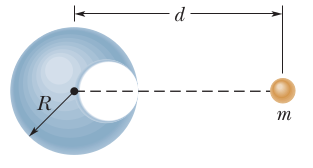
\includegraphics[scale=0.5]{./img/p4.png}
			\label{p4}
		\end{figure}
	\end{ejercicio}



\begin{ejercicio}
	Encuentre una expresión que modele el valor de $g$ dentro de la tierra, asumiendo que es una esfera uniforme.
\end{ejercicio}



\begin{ejercicio}
		Dos estrellas de masa $M$ y $m$, separadas una distancia $d$, dan vueltas en órbitas circulares en torno a su centro de masa. Demuestre que cada estrella tiene un periodo dado por
			$$ T^2 = \frac{4\pi ^2 d^3}{G (M + m)}. $$
	\end{ejercicio}



\section*{Movimiento Oscilatorio}

\begin{ejercicio}
		Una varilla metálica delgada y uniforme con masa $M$ pivota sin fricción sobre un eje que pasa por su punto medio y es perpendicular a la varilla. Un resorte horizontal con constante de fuerza $k$ se conecta al extremo inferior de la varilla, y el otro extremo del resorte se fija a un soporte rígido. La varilla se desplaza un ángulo pequeño $\theta$ conrespecto a la vertical y se suelta. Demuestre que se mueve en MAS angular y calcule su periodo.
		
		\begin{figure}[H]
			\centering
			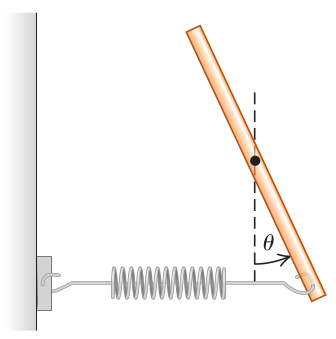
\includegraphics[scale=0.3]{./img/ej1.png}
		\end{figure}
	\end{ejercicio}




\begin{ejercicio}
		Imagine que a través del centro de la Tierra, se cava un hoyo que sale hasta el otro lado y usted, masa $m$, se lanza hacia él. Demuestre que tendrá un movimiento armónico simple si se mueve sin fricción. ¿Cuándo llegará al otro lado de la Tierra?
	\end{ejercicio}




\begin{ejercicio}
	Encuentre el periodo de oscilación de una esfera sólida de masa $M$ y radio $R$ respecto a un punto en su superficie.
\end{ejercicio}






\begin{ejercicio}
	Considere un oscilador armónico de masa $m$, constante elástica $k$ y longitud natural $L_o$, que está oscilando en presencia del campo gravitatorio creado por una esfera fija de masa $M$. La elongación del resorte en cualquier instante es $x(t)$. La distancia entre las masas $M$ y $m$ cuando el resorte no está estirado es $L$. Considerando n régimen de pequeñas oscilaciones, se cumple siempre que $L \gg x(t)$.
	\begin{figure}[H]
		\centering
		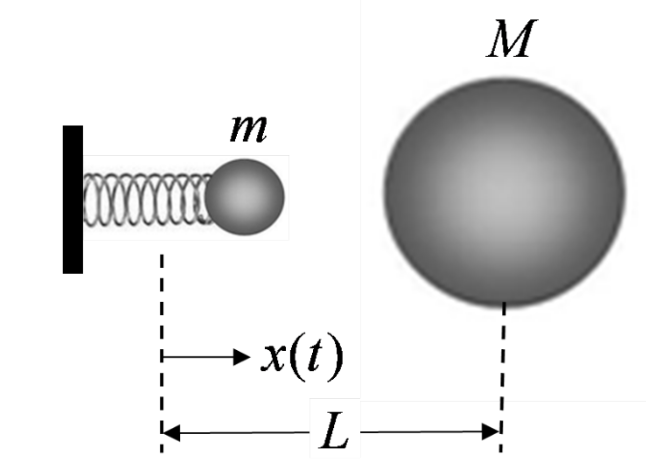
\includegraphics[scale=0.3]{./img/megabolas.png}
		\label{megabolas}
	\end{figure}
	\begin{itemize}
		\item En ausencia de la esfera de masa $M$
		\begin{enumerate}[a)]
			\item Escriba la ecuación de movimiento de la masa $m$ e indique la frecuencia natural $\omega _o$ de oscilación y la posición de equilibrio $x_o$.
		\end{enumerate}
		\item En presencia de la esfera de masa $M$
		\begin{enumerate}[a)]
			\item Escriba la ecuación de movimiento de la masa $m$.
			\item Obtenga expresiones para la nueva frecuencia angular $\omega$ y la nueva posición de equilibrio $x' _o$.
			\item Suponiendo que se miden experimentalmente $\omega$ y $x'_o$ encuentre una expresión para la constante gravitacional $G$ en función de estas magnitudes y de $L$ y $M$.
		\end{enumerate}
	\end{itemize}
	{\textit Hint: Utilize la aproximación: $(L - x)^2 \approx L^{-2} + 2xL^{-3}$, válida para $x\ll L$.}
\end{ejercicio}


































%%%%